\documentclass[aspectratio=169,10pt]{beamer}

\usetheme{Madrid}
\usecolortheme{seahorse}

\usepackage[utf8]{inputenc}
\usepackage{amsmath}
\usepackage{amssymb}
\usepackage{amsfonts}
\usepackage{mathtools}
\usepackage{listings}
\usepackage{xcolor}
\usepackage{hyperref}
\usepackage{graphicx}
\usepackage{fancybox}

\graphicspath{{figures/}}

% Listings configuration
\lstset{
    basicstyle=\ttfamily\scriptsize,
    keywordstyle=\color{blue},
    commentstyle=\color{green!50!black}\itshape,
    stringstyle=\color{red},
    showstringspaces=false,
    breaklines=true,
    frame=single,
    numbers=left,
    numberstyle=\tiny\color{gray},
    captionpos=b,
    language=Python
}

% Custom commands
\newcommand{\norm}[1]{\left\lVert#1\right\rVert}
\newcommand{\ip}[2]{\langle#1,#2\rangle}
\newcommand{\set}[1]{\left\{#1\right\}}
\newcommand{\reals}{\mathbb{R}}
\newcommand{\hilbert}{\mathcal{H}}
\newcommand{\prob}{\mathbb{P}}
\newcommand{\expectation}{\mathbb{E}}

% Beamer configuration
\setbeamertemplate{footline}[frame number]
\setbeamertemplate{navigation symbols}{}
\setbeamercovered{transparent}

\title[Fixed Point Theorems: Brouwer and Schauder]{Fixed Point Theorems of Brouwer and Schauder}
\subtitle{Pathak: An Introduction to Nonlinear Analysis and Fixed Point Theory}
\subtitle{Chapter 5, Section 5.3: Pages 309--328}
\author{Lecture Notes}
\date{\today}

\begin{document}

% Title page
\begin{frame}
    \titlepage
    \vspace{-0.5cm}
    \begin{center}
        \textbf{Key Topics:}
        \begin{itemize}
            \item Nonexpansive and Asymptotically Nonexpansive Mappings
            \item Brouwer's Fixed Point Theorem
            \item Schauder's Fixed Point Theorem
            \item Applications and Extensions
        \end{itemize}
    \end{center}
\end{frame}

% Table of contents
\begin{frame}{Outline}
    \tableofcontents
\end{frame}

% ============================================================================
\section{Preliminaries: Mapping Types}
% ============================================================================

\begin{frame}{Basic Definitions: Contractive Mappings}
    \textbf{Definition 5.23 (Pseudocontractive Mapping)}

    Let $K$ be a nonempty subset of a normed linear space $X$. A mapping $F: K \to X$ is said to be \textbf{pseudocontractive} if for each $k > 0$ and for all $x, y \in K$:
    \[
        \norm{x - y} \leq \norm{(1 + k)(x - y) - k(Fx - Fy)}.
    \]

    \vspace{0.3cm}
    In a real Hilbert space, this is equivalent to:
    \[
        \norm{Fx - Fy}^2 \leq \norm{x - y}^2 + \norm{(I - F)(x) - (I - F)(y)}^2 \quad \forall x, y \in K.
    \]

    \vspace{0.3cm}
    \textbf{Alternative form:}
    \[
        (Fx - Fy, x - y) \leq \norm{x - y}^2 \quad \forall x, y \in X.
    \]

    \vspace{0.2cm}
    \emph{Significance:} Pseudocontractive mappings are important in nonlinear analysis due to their connection with accretive operators.
\end{frame}

\begin{frame}{Nonexpansive Mappings}
    \textbf{Definition:} A mapping $T: K \to K$ is \textbf{nonexpansive} if
    \[
        \norm{Tx - Ty} \leq \norm{x - y} \quad \forall x, y \in K.
    \]

    \vspace{0.4cm}
    \textbf{Key Properties:}
    \begin{enumerate}
        \item Lipschitz constant = 1
        \item Does not require contraction
        \item Fixed point may not be unique
        \item Exists under restrictive conditions (e.g., star-shaped sets in Hilbert spaces)
    \end{enumerate}

    \vspace{0.3cm}
    \textbf{Theorem 5.40 (Kirk)} Let $\hilbert$ be a real Hilbert space and $K$ a closed star-shaped subset of $\hilbert$. Suppose $F: K \to \hilbert$ is nonexpansive with $F(\partial K) \subset K$ and $\{F^n(x_0)\}$ is bounded. Then $F$ has a fixed point.
\end{frame}

\begin{frame}{Asymptotically Nonexpansive Mappings}
    \textbf{Definition 5.24} A mapping $T: K \to K$ is \textbf{asymptotically nonexpansive} if
    \[
        \norm{T^n x - T^n y} \leq k_n \norm{x - y} \quad \forall x, y \in K \quad \text{and} \quad \lim_{n\to\infty} k_n = 1.
    \]

    \vspace{0.3cm}
    \textbf{Definition 5.25} A mapping $T: K \to K$ is \textbf{asymptotically regular} if for any $x \in K$,
    \[
        \norm{T^n x - T^{n+1} x} \to 0 \quad \text{as } n \to \infty.
    \]

    \vspace{0.4cm}
    \textbf{Theorem 5.42 (Goebel and Kirk, 1972)} Let $K$ be nonempty, closed, convex and bounded subset of a uniformly convex Banach space and let $T$ be an asymptotically nonexpansive mapping of $K$ into itself. Then $T$ has a fixed point in $K$.

    \vspace{0.2cm}
    This is a major extension of the Brouwer fixed point theorem to infinite-dimensional settings.
\end{frame}

\begin{frame}{Comparison of Mapping Types}{Visual Illustration}
    \begin{center}
        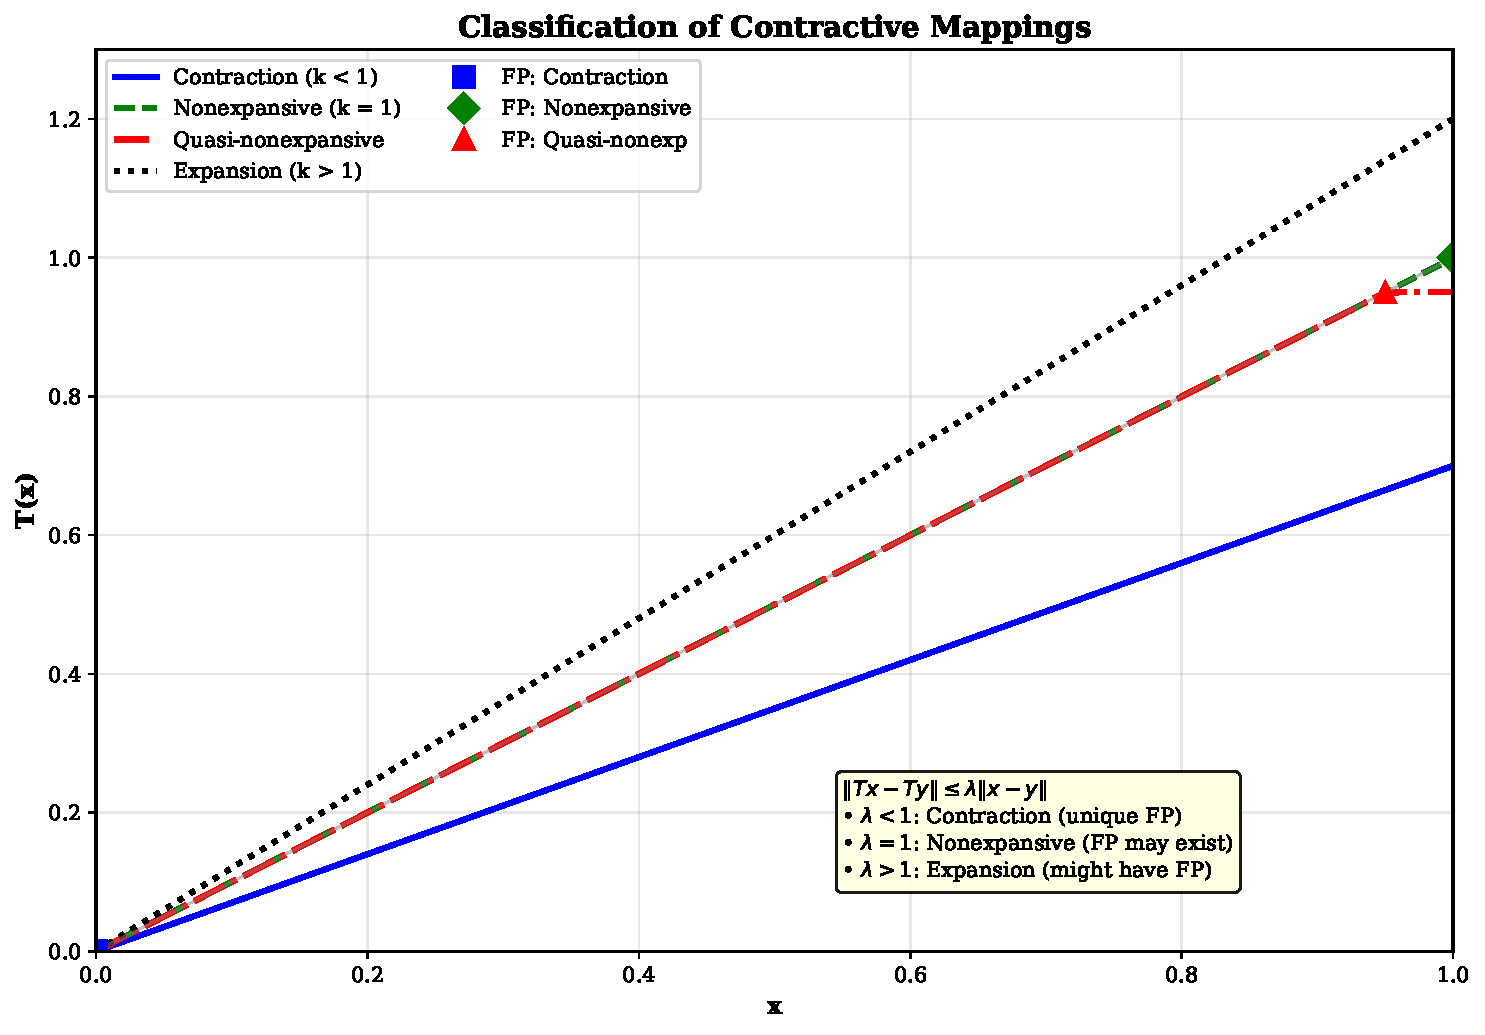
\includegraphics[width=0.9\textwidth]{fig_contraction_mapping.pdf}
    \end{center}

    \vspace{-0.3cm}
    \footnotesize
    \textbf{Classification:}
    \begin{itemize}
        \item \textcolor{blue}{Contraction ($k < 1$):} Always has unique fixed point (Banach)
        \item \textcolor{green}{Nonexpansive ($k = 1$):} May have fixed point (requires conditions)
        \item \textcolor{red}{Quasi-nonexpansive:} Intermediate behavior
        \item Black dashed: Expansion ($k > 1$)
    \end{itemize}
\end{frame}

% ============================================================================
\section{Brouwer's Fixed Point Theorem}
% ============================================================================

\begin{frame}{Brouwer's Fixed Point Theorem}{Fundamental Result}
    \textbf{Theorem 5.48 (Brouwer's Fixed Point Theorem)}

    The closed unit ball $\mathbb{B}^n = \{x \in \mathbb{R}^n : \|x\| \leq 1\}$ of $\mathbb{R}^n$ has the \textbf{fixed point property}.

    Alternatively: Let $f: \mathbb{B}^n \to \mathbb{B}^n$ be a continuous function. Then $f$ has a fixed point $\bar{x} \in \mathbb{B}^n$.

    \vspace{0.4cm}
    \textbf{Historical Note:}
    \begin{itemize}
        \item Brouwer: 1910 (first complete proof for $n = 3$)
        \item Poincaré: 1886 (different version)
        \item Brouwer: 1912 (proof for arbitrary $n$)
    \end{itemize}

    \vspace{0.3cm}
    \textbf{Limitations:}
    \begin{itemize}
        \item Does NOT provide computational scheme
        \item Does NOT guarantee uniqueness
        \item Limited to finite dimensions (needs modification for infinite dimensions)
    \end{itemize}
\end{frame}

\begin{frame}{Brouwer's Theorem: Geometric Interpretation}{Topological Proof Sketch}
    \begin{center}
        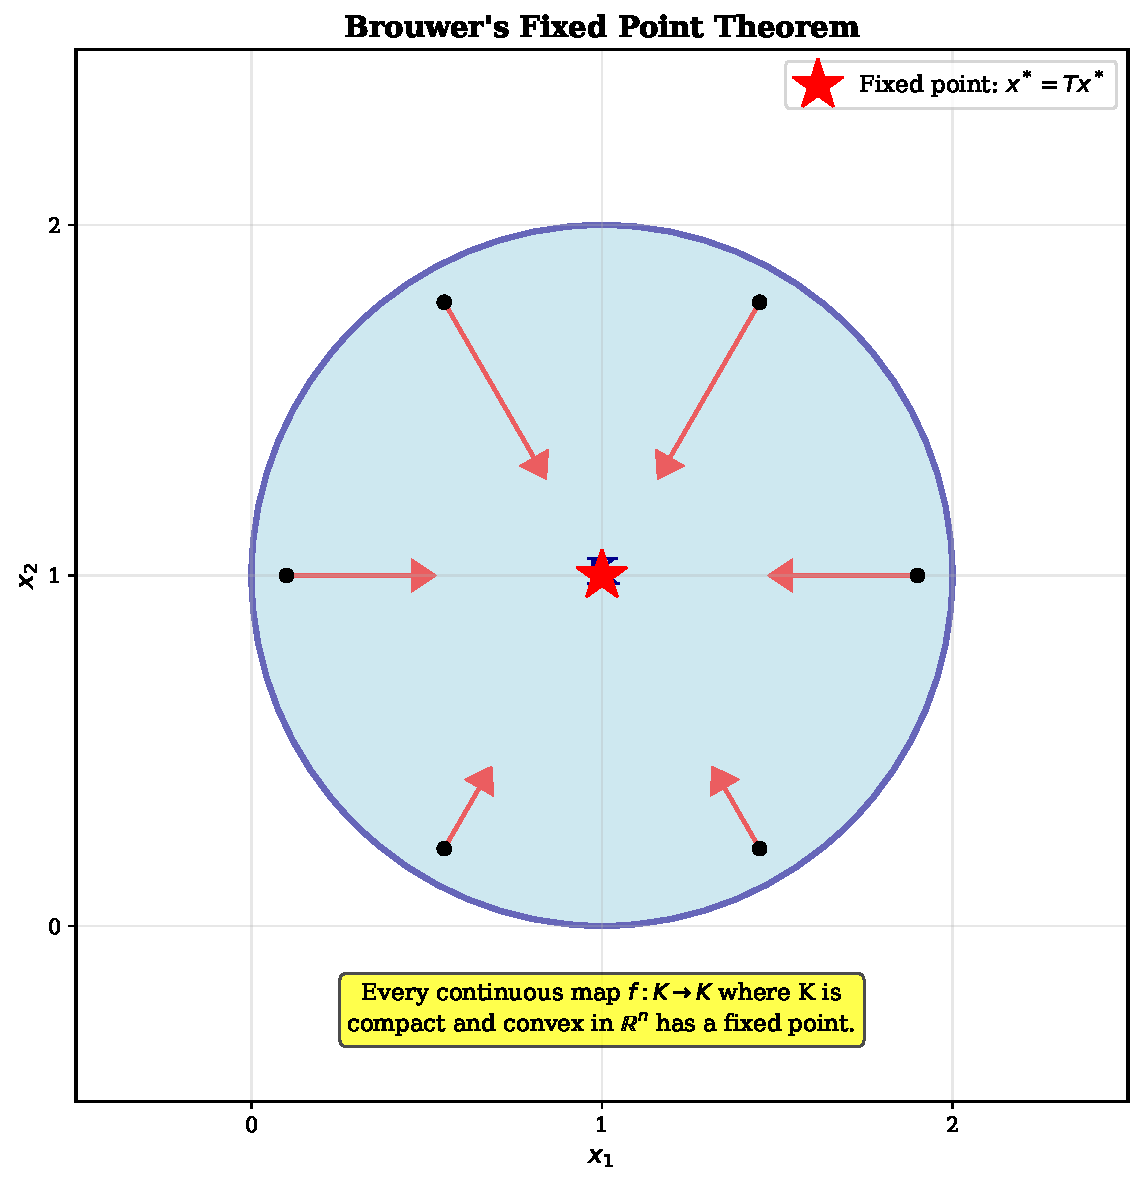
\includegraphics[width=0.85\textwidth]{fig_brouwer_fixed_point.pdf}
    \end{center}

    \vspace{0.2cm}
    \textbf{Key Idea:} The theorem relies on:
    \begin{itemize}
        \item Algebraic topology (homology groups)
        \item Retraction concepts from differential forms
        \item $S^{n-1}$ is NOT a retract of $\mathbb{B}^n$
    \end{itemize}
\end{frame}

\begin{frame}[allowframebreaks]{Lemma 5.7: Topological Foundation}
    \textbf{Lemma 5.7} The set $S^{n-1} = \{x \in \mathbb{R}^n : \|x\| = 1\}$ is not a retract of $\mathbb{B}^n$.

    \vspace{0.3cm}
    \textbf{Proof Sketch (using Algebraic Topology):}

    A retraction $r: \mathbb{B}^n \to S^{n-1}$ would induce a homomorphism:
    \[
        r_*: H_{n-1}(\mathbb{B}^n) \to H_{n-1}(S^{n-1})
    \]

    \begin{itemize}
        \item Natural injection: $j: S^{n-1} \to \mathbb{B}^n$ induces $j_*$
        \item Composition: $(r \circ j)_* = r_* \circ j_*$ is the identity on $H_{n-1}(S^{n-1})$
        \item But: $H_{n-1}(\mathbb{B}^n) = 0$ (ball is contractible)
        \item While: $H_{n-1}(S^{n-1}) = \mathbb{Z}$ (sphere has nontrivial homology)
        \item Contradiction!
    \end{itemize}

    \framebreak

    \textbf{Analytical Proof (using Differential Forms):}

    Associate to $C^2$ function $h: \mathbb{B}^n \to \mathbb{B}^n$ the exterior form:
    \[
        \omega_h = h_1 dh_2 \wedge \cdots \wedge dh_n
    \]

    By Stokes theorem:
    \[
        \int_{S^{n-1}} \omega_h = \int_{\mathbb{B}^n} d\omega_h = \int_{\mathbb{B}^n} \det[J_h(x)] dx
    \]

    If retraction $r$ of class $C^2$ existed, then $\det[J_r] \equiv 0$, so:
    \[
        \int_{S^{n-1}} \omega_r = 0
    \]

    But $r|_{S^{n-1}} = i_{S^{n-1}}$ (identity), so integral must equal volume of $S^{n-1}$. Contradiction!
\end{frame}

\begin{frame}[fragile]{Application: Numerical Example}{Fixed Point Iteration}
    \textbf{Problem:} Find fixed point of $f(x) = 0.5x + 0.3$ on $\mathbb{B}^1 = [-1, 1]$.

    \begin{columns}[T]
        \column{0.5\textwidth}
        \begin{lstlisting}
import numpy as np
import matplotlib.pyplot as plt

def f(x):
    return 0.5 * x + 0.3

# Fixed point iteration
x_init = 0.1
x_seq = [x_init]
for i in range(10):
    x_new = f(x_seq[-1])
    x_seq.append(x_new)

x_seq = np.array(x_seq)

# Exact fixed point: x* = 0.5*x* + 0.3
x_star = 0.6

print(f"Iterations: {x_seq}")
print(f"Fixed point: {x_star}")
print(f"Final error: {abs(x_seq[-1] - x_star)}")
        \end{lstlisting}

        \column{0.5\textwidth}
        \begin{center}
            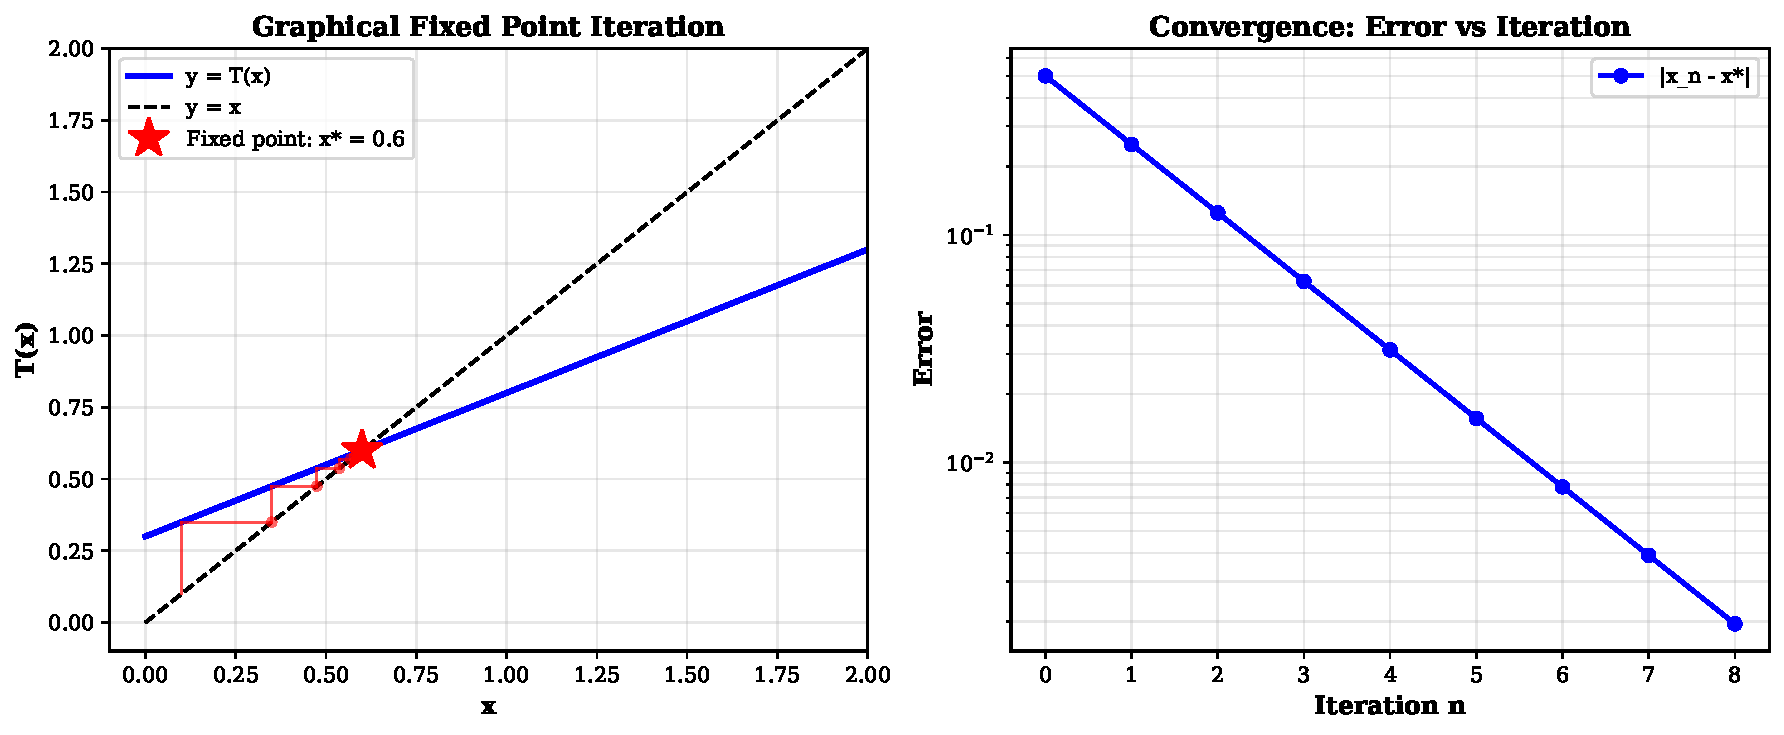
\includegraphics[width=0.95\textwidth]{fig_fixed_point_iteration.pdf}
        \end{center}

        \vspace{-0.3cm}
        \textbf{Output:}
        \begin{itemize}
            \item Iterations converge to $x^* = 0.6$
            \item Exponential error decay
            \item By Brouwer: $\exists x^* : f(x^*) = x^*$
        \end{itemize}
    \end{columns}
\end{frame}

% ============================================================================
\section{Schauder's Fixed Point Theorem}
% ============================================================================

\begin{frame}{Schauder's Fixed Point Theorem}{Extension to Infinite Dimensions}
    \textbf{Theorem 5.54 (Schauder's Fixed Point Theorem)}

    Let $X$ be a Banach space, $K$ a nonempty, closed and convex subset of $X$, and $T: K \to K$ a continuous mapping. If $T(K)$ is relatively compact in $K$, then $T$ has a fixed point in $K$.

    \vspace{0.4cm}
    \textbf{Corollary 5.11:} If $K$ is compact and convex, and $T: K \to K$ is continuous, then $T$ has a fixed point.

    \vspace{0.3cm}
    \textbf{Key Advantage over Brouwer:}
    \begin{itemize}
        \item Works in \textbf{infinite-dimensional} spaces
        \item Applies to more general settings (Fréchet spaces, etc.)
        \item No restriction to finite balls
    \end{itemize}

    \vspace{0.3cm}
    \textbf{Comparison with Brouwer:}
    \begin{center}
        \begin{tabular}{l|cc}
            Property & Brouwer & Schauder \\
            \hline
            Finite dimension & Yes & Yes \\
            Infinite dimension & No & \textbf{Yes} \\
            Compact domain & No (ball OK) & \textbf{Yes} \\
            Convex domain & Yes & Yes \\
        \end{tabular}
    \end{center}
\end{frame}

\begin{frame}{Schauder's Theorem: Key Concepts}{Relative Compactness and Continuous Mappings}
    \begin{center}
        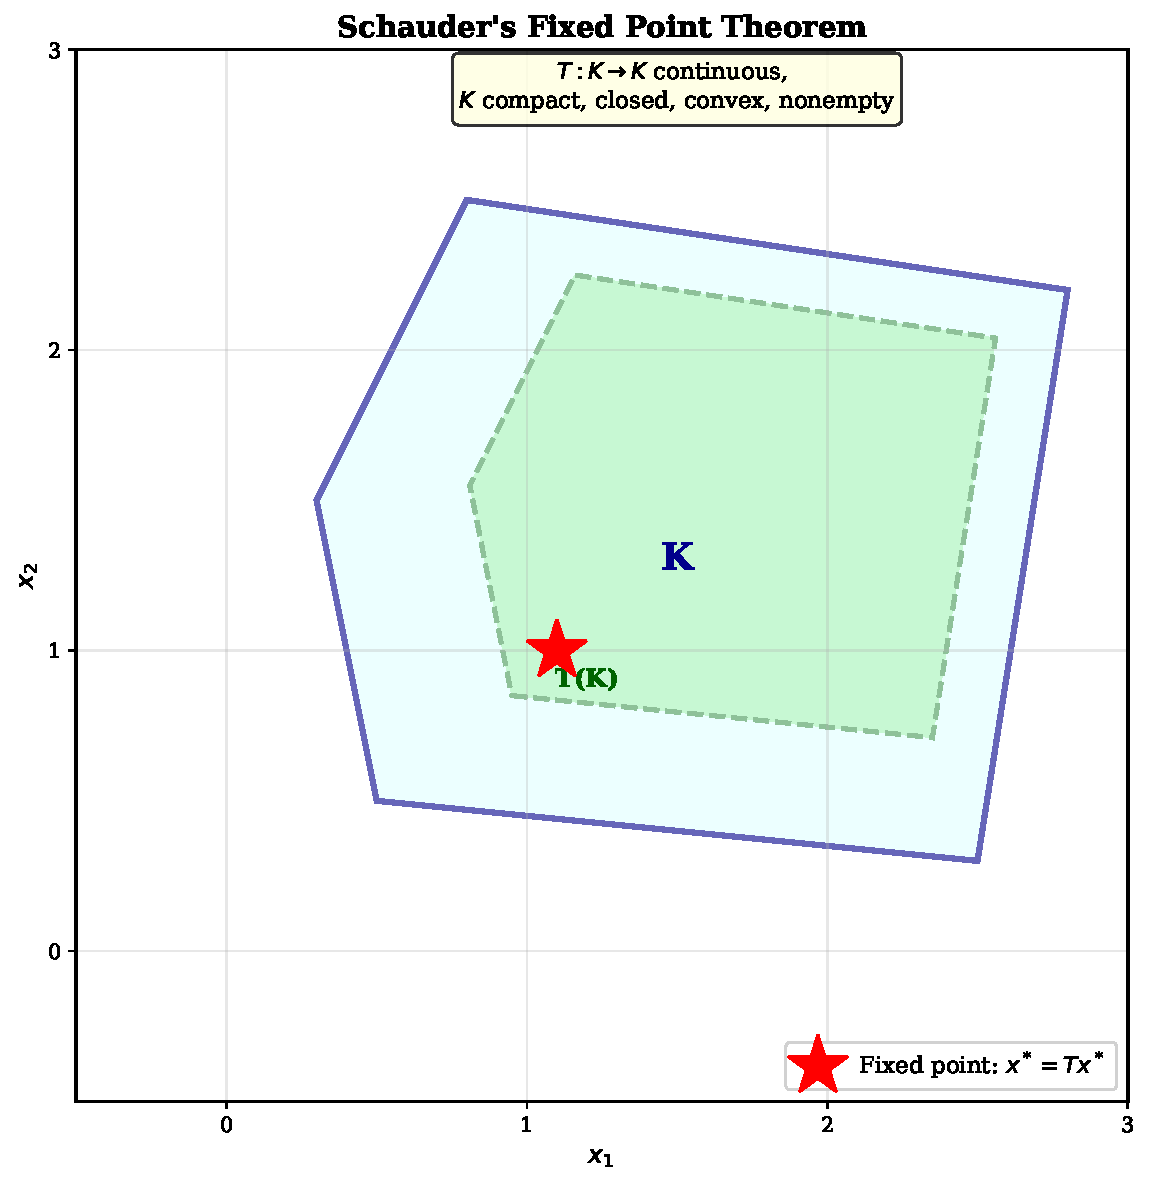
\includegraphics[width=0.85\textwidth]{fig_schauder_fixed_point.pdf}
    \end{center}

    \vspace{0.2cm}
    \textbf{Essential Conditions:}
    \begin{enumerate}
        \item $K$ is \textbf{nonempty and convex}
        \item $T: K \to K$ is \textbf{continuous}
        \item $T(K)$ is \textbf{relatively compact} (closure is compact)
    \end{enumerate}

    \textbf{Note:} Condition (c) may be interpreted as \textit{asymptotic regularity} under certain hypotheses.
\end{frame}

\begin{frame}[allowframebreaks]{Theorem 5.55: Schauder's Theorem (Finite Dimension Version)}
    \textbf{Theorem 5.55} Let $K$ be a nonempty, compact and convex subset of a Banach space $X$ and let $T$ be a continuous mapping of $K$ into itself. Then $T$ has a fixed point in $K$.

    \vspace{0.4cm}
    \textbf{Proof Outline:}

    \begin{enumerate}
        \item By Theorem 5.52: Any compact convex set $K$ is homeomorphic to a compact convex subset $C$ of some $\mathcal{H}_0$ (Hilbert cube)

        \item By Theorem 5.54: $C$ has the fixed point property

        \item By Theorem 5.45: $K$ has the fixed point property

        \item Therefore $T$ has a fixed point in $K$
    \end{enumerate}

    \framebreak

    \textbf{Theorem 5.56:} Let $K$ be a nonempty, compact and convex subset of a normed linear space $X$ and let $T$ be a continuous mapping of $K$ into itself. Then $T$ has a fixed point in $K$.

    \vspace{0.3cm}
    \textbf{Theorem 5.57:} Let $T$ be a compact and continuous mapping of a normed linear space $X$ into itself and let $T(X)$ be bounded. Then $T$ has a fixed point.

    \vspace{0.3cm}
    \textbf{Proof:} Let $K$ be the closed and convex hull of $T(X)$. Then $K$ is bounded and $T(K) \subset K$. By Theorem 5.55 $T$ has a fixed point in $K$. $\square$
\end{frame}

\begin{frame}[allowframebreaks]{Theorem 5.58: Reflexive Banach Spaces}
    \textbf{Theorem 5.58} Let $X$ be a reflexive Banach space, $K$ a closed and convex subset of $X$ and $T$ a weakly continuous mapping of $K$ into a bounded subset of $K$. Then $T$ has a fixed point in $K$.

    \vspace{0.3cm}
    \textbf{Key Points:}
    \begin{itemize}
        \item Extends Schauder to \textbf{reflexive} spaces
        \item Uses weak compactness instead of norm compactness
        \item Weakly continuous: If $x_n \rightharpoonup x$, then $Tx_n \rightharpoonup Tx$
        \item Applies to $L^p$ spaces ($1 < p < \infty$)
    \end{itemize}

    \framebreak

    \textbf{Theorem 5.63 (Potter [491])} Let $X$ be a normed linear space. Let $K$ be any closed and convex subset of $X$ and $T$ be a continuous mapping of $K$ into a compact subset of $X$ such that $T(\partial K) \subset K$. Then $T$ has a fixed point.

    \vspace{0.3cm}
    \textbf{Proof Idea:}
    \begin{itemize}
        \item Define radial retraction $R$ of $X$ onto $K$
        \item Map $RT: K \to K$ is continuous into compact set
        \item By Schauder: $RT$ has fixed point $u \in K$
        \item Can show this $u$ is fixed point of $T$
    \end{itemize}
\end{frame}

% ============================================================================
\section{Key Extensions and Variations}
% ============================================================================

\begin{frame}{Theorem 5.41: Lipschitzian Pseudocontractive Mappings}
    \textbf{Theorem 5.41 (Kirk and Ray [334])} Let $K$ be a closed and convex subset of a uniformly convex Banach space $X$. Let $F: K \to K$ be a Lipschitzian pseudocontractive mapping. Suppose for some $a \in K$, the set
    \[
        G(a, Fa) = \set{z \in K : \norm{z - a} \geq \norm{z - Fa}}
    \]
    is bounded. Then $F$ has a fixed point in $K$.

    \vspace{0.3cm}
    \textbf{Proof Strategy:}
    \begin{enumerate}
        \item For each $y \in K$, define $F_y(x) = (1-\alpha)y + \alpha F(F_y(y)), x \in K$
        \item Show $F_y$ is a contraction for appropriate $\alpha \in (0, 1)$
        \item Obtain fixed point $T_a(y)$ of $F_y$
        \item Prove that fixed point of $T_a$ gives fixed point of $F$
    \end{enumerate}
\end{frame}

\begin{frame}{Theorem 5.65: Potter's Result}{Geometric Conditions}
    \textbf{Theorem 5.65 (Potter [491])} Let $X$ be a normed linear space. Let $K$ be any closed and convex subset of $X$ and $T$ be a continuous mapping of $K$ into a compact subset of $X$ such that $T(\partial K) \subset K$. Then $T$ has a fixed point.

    \vspace{0.4cm}
    \textbf{Geometric Interpretation:}
    \begin{itemize}
        \item The boundary condition $T(\partial K) \subset K$ ensures:
        \begin{itemize}
            \item No fixed point can lie on $\partial K$ (boundary)
            \item Continuous extension into interior
            \item Topological degree argument applies
        \end{itemize}
        \item Radial retraction $R(x) = \frac{x}{\max(1, \rho(x))}$ defines mapping $RT$
        \item $RT$ inherits fixed point property from Schauder
    \end{itemize}
\end{frame}

\begin{frame}{The Schauder-Tychonoff Fixed Point Theorem}{Generalization to Locally Convex Spaces}
    \textbf{Theorem 5.54 (Schauder-Tychonoff)}

    Let $X$ be a locally convex topological vector space, $K$ a nonempty compact convex subset of $X$, and $T: K \to K$ a continuous mapping. Then $T$ has a fixed point in $K$.

    \vspace{0.3cm}
    \textbf{Remark 5.25:} This theorem generalizes Brouwer's result from finite-dimensional spaces to:
    \begin{itemize}
        \item Banach spaces (with compactness condition)
        \item Fréchet spaces
        \item Locally convex topological vector spaces
        \item Even infinite-dimensional normed spaces
    \end{itemize}

    \vspace{0.3cm}
    \textbf{Lemma 5.8:} Every continuous function $f: K \to K$ on finite-dimensional compact convex set has a fixed point.

    \begin{itemize}
        \item Extension step uses Tychonoff's compactness theorem
        \item Finite-dimensional projections inherit fixed points
        \item Limiting argument gives fixed point in full space
    \end{itemize}
\end{frame}

% ============================================================================
\section{Asymptotically Nonexpansive Mappings}
% ============================================================================

\begin{frame}{Asymptotically Nonexpansive Mappings: Detailed Analysis}
    \textbf{Definition 5.24 and 5.27} A sequence $\{T_n\}$ of self-mappings of $K$ is \textbf{asymptotically nonexpansive} if:
    \[
        \norm{T_n x - T_n y} \leq k_n \norm{x - y} \quad \forall x, y \in K, \quad \lim_{n\to\infty} k_n = 1.
    \]

    \vspace{0.3cm}
    \begin{center}
        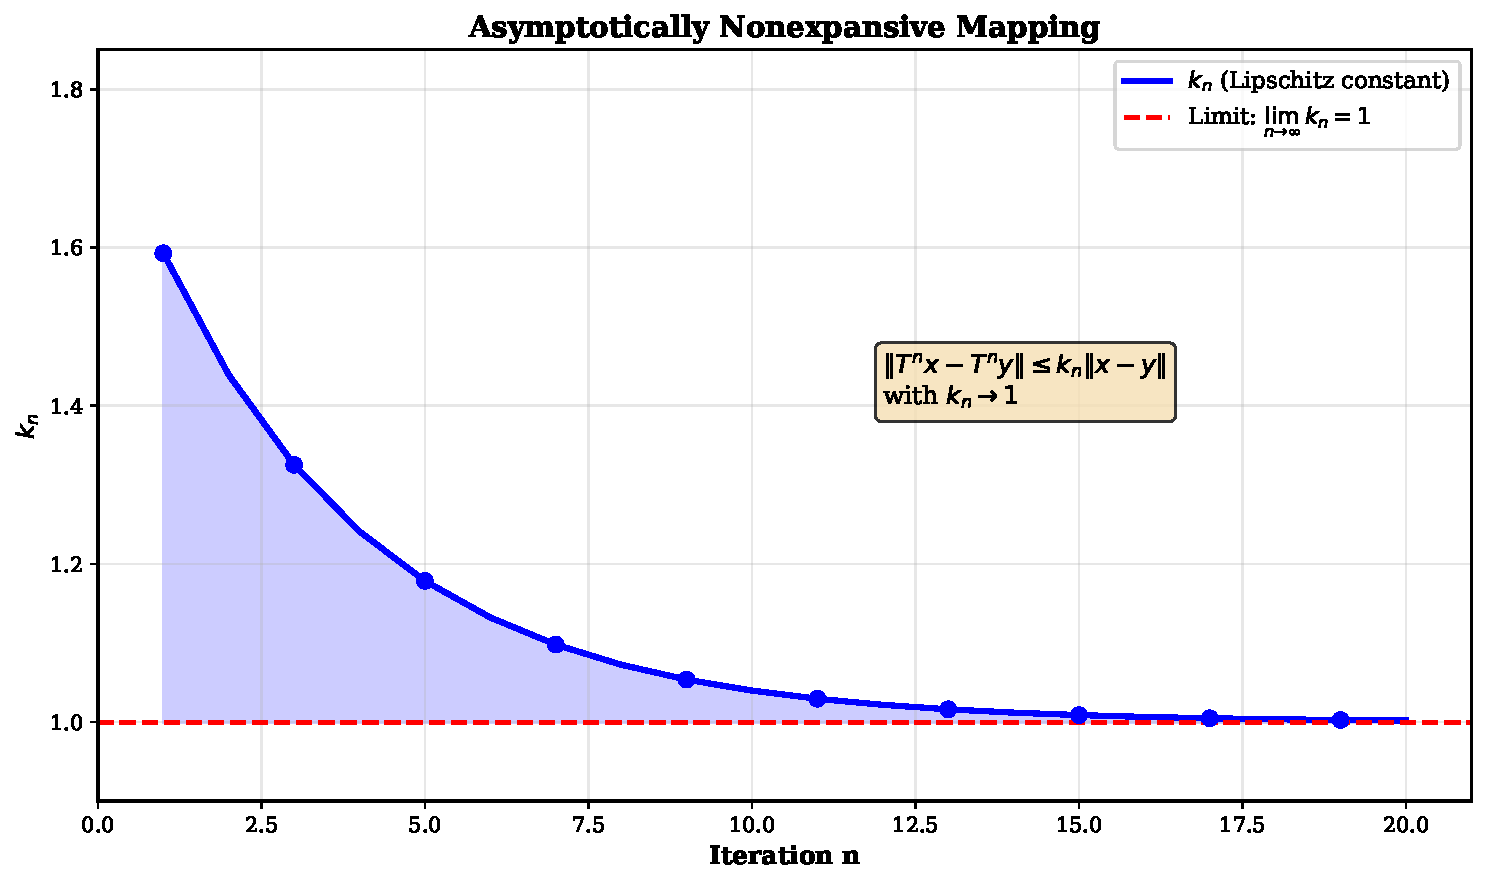
\includegraphics[width=0.9\textwidth]{fig_asymptotically_nonexpansive.pdf}
    \end{center}

    \vspace{0.2cm}
    \textbf{Key Observation:} The Lipschitz constant approaches 1, but never equals it. This is intermediate between:
    \begin{itemize}
        \item Nonexpansive mappings: $k_n = 1$ for all $n$
        \item Asymptotically regular: $\norm{T^nx - T^{n+1}x} \to 0$
    \end{itemize}
\end{frame}

\begin{frame}{Theorem 5.44: Asymptotically Nonexpansive Sequences}{Main Convergence Result}
    \textbf{Theorem 5.44} Let $X$ be a uniformly convex Banach space with Fréchet differentiable norm and $K$ a closed and convex subset of $X$. Let $C$ be a subset of $K$ and $S = \{T_n\}_{n=1}^{\infty}$, an asymptotically nonexpansive sequence of self-mappings of $K$ such that

    \begin{enumerate}
        \item $C \subset \bigcap_{n=1}^{\infty} \mathcal{F}(T_n)$
        \item There exists $x_0 \in K$ for which $T_{n_k} x_0 \to z$ implies that $z \in C$
        \item $T_n T_m x_0 - T_n x_0 \to 0$ as $n \to \infty$ for all (fixed) $m$
    \end{enumerate}

    Then either:
    \begin{enumerate}
        \item $C = \emptyset$ and $\norm{T_n x_0} \to +\infty$, or
        \item $C \neq \emptyset$ and $T_n x_0$ converges weakly to an element of $C$.
    \end{enumerate}

    \textbf{Note:} Hypothesis (c) is asymptotic regularity at $x_0$.
\end{frame}

\begin{frame}[fragile]{Numerical Example: Asymptotic Behavior}{Python Implementation}
    \begin{columns}[T]
        \column{0.55\textwidth}
        \begin{lstlisting}
import numpy as np

# Asymptotically nonexpansive map
def T_n(x, n):
    """T_n(x) with k_n = 1 + exp(-n/10)"""
    k_n = 1.0 + np.exp(-n/10.0)
    # Example: contraction with varying rate
    return k_n * 0.5 * x

# Sequence of mappings
x0 = 1.0
x_history = [x0]
k_history = []

for n in range(1, 51):
    k_n = 1.0 + np.exp(-n/10.0)
    k_history.append(k_n)
    x_new = T_n(x_history[-1], n)
    x_history.append(x_new)

x_history = np.array(x_history)
k_history = np.array(k_history)

# Analysis
print("k_n values:", k_history[-5:])
print("x_n values:", x_history[-5:])
print("Convergence to 0")
        \end{lstlisting}

        \column{0.45\textwidth}
        \textbf{Properties Observed:}
        \begin{itemize}
            \item $k_n \to 1$ as $n \to \infty$
            \item Sequence $\{x_n\}$ converges
            \item Rate of convergence depends on $k_n$
            \item Slower than exponential for small $n$
            \item Eventually linear rate
        \end{itemize}

        \vspace{0.3cm}
        \textbf{Theorem 5.42 Guarantee:}
        Under suitable conditions (uniformly convex Banach space, bounded set), asymptotically nonexpansive mappings have fixed points.
    \end{columns}
\end{frame}

% ============================================================================
\section{Summary and Applications}
% ============================================================================

\begin{frame}{Summary: Fixed Point Theorems Hierarchy}
    \textbf{Classification by Generality:}

    \begin{enumerate}
        \item \textbf{Banach Contraction Mapping Principle}
            \begin{itemize}
                \item Requires: $\norm{Tx - Ty} \leq \lambda\norm{x-y}$, $\lambda < 1$
                \item Guarantees: Unique fixed point + computational scheme
            \end{itemize}

        \item \textbf{Brouwer's Fixed Point Theorem}
            \begin{itemize}
                \item Requires: Continuous map, compact convex set in $\mathbb{R}^n$
                \item Guarantees: Fixed point exists (no uniqueness, no algorithm)
            \end{itemize}

        \item \textbf{Schauder's Fixed Point Theorem}
            \begin{itemize}
                \item Requires: Continuous map, compact convex set in Banach space
                \item Guarantees: Fixed point exists in infinite dimensions
            \end{itemize}

        \item \textbf{Nonexpansive/Asymptotically Nonexpansive}
            \begin{itemize}
                \item Requires: Lipschitz constant $\geq 1$, special spaces
                \item Guarantees: Fixed points under structural conditions
            \end{itemize}
    \end{enumerate}
\end{frame}

\begin{frame}{Applications and Significance}{From Theory to Practice}
    \textbf{Mathematical Applications:}
    \begin{itemize}
        \item \textbf{Differential Equations:} Existence of solutions via fixed points of integral operators
        \item \textbf{Optimization:} Finding minimizers of convex functionals
        \item \textbf{Game Theory:} Nash equilibrium points (Kakutani's theorem uses fixed points)
        \item \textbf{Functional Analysis:} Extending results to infinite-dimensional spaces
    \end{itemize}

    \vspace{0.3cm}
    \textbf{Computational Methods:}
    \begin{itemize}
        \item \textbf{Fixed point iteration:} $x_{n+1} = T(x_n)$
        \item \textbf{Krasnoselski iteration:} $x_{n+1} = (1-\lambda)x_n + \lambda T(x_n)$
        \item \textbf{Mann iteration:} Weighted averages of iterates
        \item \textbf{Convergence analysis:} Error bounds from Lipschitz constants
    \end{itemize}

    \vspace{0.3cm}
    \textbf{Physical Applications:}
    \begin{itemize}
        \item Bifurcation theory in dynamical systems
        \item Equilibrium solutions in mechanics
        \item Variational inequalities in PDEs
    \end{itemize}
\end{frame}

\begin{frame}{Open Problems and Extensions}
    \textbf{Areas of Active Research:}
    \begin{enumerate}
        \item \textbf{Computational Complexity:}
            \begin{itemize}
                \item Efficient algorithms for finding fixed points
                \item Approximation schemes for nonexpansive mappings
            \end{itemize}

        \item \textbf{Generalized Spaces:}
            \begin{itemize}
                \item Fixed points in metric spaces with partial metrics
                \item Fixed points in fuzzy metric spaces
                \item Graph metric spaces
            \end{itemize}

        \item \textbf{Coupled Fixed Points:}
            \begin{itemize}
                \item Systems of equations
                \item Multiple interacting mappings
            \end{itemize}

        \item \textbf{Stability and Robustness:}
            \begin{itemize}
                \item How do fixed points change under perturbations?
                \item Stability of iteration schemes
            \end{itemize}
    \end{enumerate}
\end{frame}

% ============================================================================
\section{References and Further Reading}
% ============================================================================

\begin{frame}{Key References}{From Pathak's Text}
    \small
    \begin{thebibliography}{10}
        \bibitem{Pathak} Pathak, H. K. (2018). \textit{An Introduction to Nonlinear Analysis and Fixed Point Theory}. Springer.

        \bibitem{Brouwer} Brouwer, L. E. J. (1910-1912). Fixed point theorems in $\mathbb{R}^n$.

        \bibitem{Kirk} Kirk, W. A., \& Schoenberg, R. (1972). Fixed point theorems for various classes of mappings.

        \bibitem{Goebel} Goebel, K., \& Kirk, W. A. (1972). A fixed point theorem for asymptotically nonexpansive mappings. \textit{Proc. Amer. Math. Soc.}, 35, 171-174.

        \bibitem{Schauder} Schauder, J. (1930). Der Fixpunktsatz in Funktionsräumen. \textit{Studia Mathematica}, 2, 171-180.
    \end{thebibliography}
\end{frame}

\begin{frame}{Conclusion}
    \begin{center}
        \Large
        \textbf{Summary of Key Results}
    \end{center}

    \vspace{0.5cm}

    \begin{itemize}
        \setlength{\itemsep}{0.3cm}

        \item \textbf{Brouwer's Theorem:} Continuous maps on compact convex sets in $\mathbb{R}^n$ have fixed points

        \item \textbf{Schauder's Theorem:} Extension to infinite-dimensional Banach spaces with appropriate compactness conditions

        \item \textbf{Nonexpansive Maps:} When $\norm{Tx-Ty} \leq \norm{x-y}$, fixed points exist under structural conditions

        \item \textbf{Asymptotically Nonexpansive:} $k_n \to 1$ provides intermediate theory between contractions and nonexpansive

        \item \textbf{Practical Impact:} These theorems guarantee existence (not always constructive) but motivate iterative algorithms

    \end{itemize}

    \vspace{0.8cm}

    \begin{center}
        \textbf{Questions?}
    \end{center}
\end{frame}

\end{document}
